% flashcards-title: Upward-positive free-fall setup
% flashcards-desc: A vertical y axis points upward from a release level to a top point; the one-dimensional motion line is dashed and a separate acceleration arrow points downward.
\documentclass[border=7pt]{standalone}
\def\pgfsysdriver{pgfsys-dvisvgm.def}
\usepackage{tikz}
\usetikzlibrary{arrows.meta,positioning,shapes.geometric}
\definecolor{mechInk}{HTML}{172033}
\definecolor{mechBlue}{HTML}{155EEF}
\definecolor{mechOrange}{HTML}{B54708}
\definecolor{mechPale}{HTML}{E8F0FF}
\definecolor{mechGray}{HTML}{667085}
\definecolor{mechLight}{HTML}{D0D5DD}
\tikzset{
  every picture/.style={font=\sffamily\large, text=mechInk},
  mech box/.style={draw=mechInk, line width=1.2pt, rounded corners=4pt,
    fill=white, align=center, minimum height=14mm, inner xsep=5mm},
  mech primary/.style={draw=mechBlue, line width=2.2pt},
  mech secondary/.style={draw=mechOrange, line width=2.2pt, dashed},
  mech guide/.style={draw=mechGray, line width=0.9pt, dashed},
  mech arrow/.style={-{Stealth[length=3.2mm,width=2.4mm]},
    draw=mechInk, line width=1.4pt, line cap=butt},
  mech axis/.style={draw=mechInk, line width=1.2pt},
  mech tick/.style={draw=mechInk, line width=1pt}
}

\begin{document}
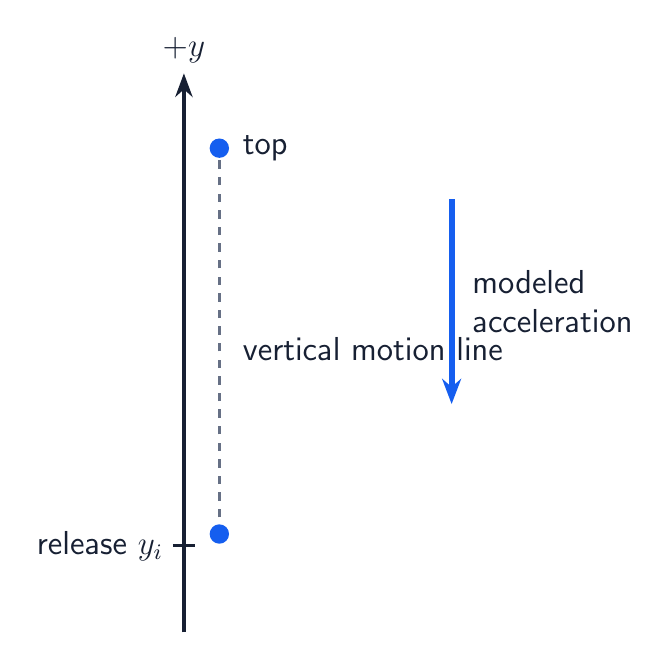
\begin{tikzpicture}[x=1cm,y=1cm]
  \draw[mech axis,-{Stealth[length=3mm,width=2.2mm]}] (0,-0.8) -- (0,6.3) node[above] {\(+y\)};
  \draw[mech tick] (-0.14,0.3) -- (0.14,0.3);
  \node[left=4pt] at (0,0.3) {release \(y_i\)};
  \draw[mech guide] (0.45,0.45) -- (0.45,5.35);
  \fill[mechBlue] (0.45,0.45) circle (3.5pt);
  \fill[mechBlue] (0.45,5.35) circle (3.5pt);
  \node[right=5pt] at (0.45,5.35) {top};
  \node[right=5pt] at (0.45,2.8) {vertical motion line};
  \draw[mech primary,-{Stealth[length=3.2mm,width=2.4mm]},line cap=butt] (3.4,4.7) -- (3.4,2.1);
  \node[right=4pt,align=left] at (3.4,3.4) {modeled\\acceleration};
\end{tikzpicture}
\end{document}
